\documentclass[11pt]{article}

\usepackage{url}
\usepackage[letterpaper,margin=1in]{geometry}
\usepackage{times}
\usepackage{graphicx}


\begin{document}

\title{Verification of Exodus}
\author{Da Yu \and Charles Yeh \and Silao Xu}
\date{Project Proposal - CSCI 2950-u - Spring 2014}
\maketitle

%\begin{abstract}
%This is the abstract. This is the abstract. This is the abstract. 
%This is the abstract. This is the abstract. This is the abstract. 
%This is the abstract. This is the abstract. This is the abstract. 
%This is the abstract. This is the abstract. This is the abstract. 
%This is the abstract. This is the abstract. This is the abstract. 
%\end{abstract}

\section{Problem Statement}
%\label{sec:intro}
%This is a simple example file on how to write a report using LaTeX.
%Just use it as a base and replace the content. I put some examples of
%commonly used features, but there are many more. Generally, you learn
%these on demand. Examples include:
\par Currently, conventional networks are becoming more and more complicated. In order to maintain normal states, routers and switches need to carry or deploy many protocols or mechanisms simultaneously such as routing algorithms, ACLs, VLANs, etc. To achieve that, network administrators need to write distributed programs on the routers in various router-configuration languages, which is very tedious and prone to mistakes. However, software-defined networking (SDN) separates the intertwined control-plane and data-plane by providing abstraction and centralized-control of the network. Instead of forcing users to program at the lowest network level and manually handle routing-configuration languages, SDNs allow people to focus on high-level logical policies.
\par Exodus is a project that migrating original networks to SDNs. It consumes router configuration files in the original networks and translate them into high-level programs, which can be compiled into OpenFlow switches by the controller. Ideally, the generated SDN will perform the same policies as those performed in the original networks. However, this has not been extensively tested or verified. We intend to extensively verify and prove that the generated network by Exodus is equivalent to the original network.

\section{Proposal}

\subsection{Challenges and Questions}
\par Packets' fate are determined by the rules installed in the switches or routers. In original networks (like Cisco IOS routers), switches and routers run a set of different algorithms or mechanisms simultaneously to maintain the forwarding table. These algorithms and mechanisms are defined in the switches' or routers' configuration files, which are programmed by the network administrator. Compared with the conventional networks, a logic-centralized controller runs these algorithms and mechanisms, which are compiled from high-level logic languages, to generate exact rules and distribute them to the switches and routers.
\par For the verification work, we have a lot of challenges and questions that need to be solved:
\begin{itemize}
\item Intuitively, a good approach to verify the equivalence of two networks is to find out the differences in their flow tables. However, it is hard to be implemented: the flow tables are dynamic: Different network contexts may results in different flow tables. In order to prove the correctness of Exodus results, we need to prove the result of Exodus should be the same with the original network at any time. Which network contexts we need to prove? How many network contexts we need to check? How to make network contexts change?
\item Another good approach is to regard the routers and switches as black boxes. What we need to check is the packets' fate in the two different networks. If they have the same fate all the time, we can conclude that these two networks are equal. However, several questions need to be answers: Since it is not possible to generate all kinds of packets, how many packets we need to generate to cover every rule in the original network and the Exodus generated one? Due to the changes of network contexts, how often should we make tests? Does the test packets set need to be modified?
\end{itemize}

\subsection{Possible Solutions}
\par Header Space Analysis(HSA) is a static checking method. It regards the whole network as composition of Network Transfer Functions($\Psi$) and Topology Transfer Function($\Gamma$). For example, a packet(p) with header(h) from Host A to Host B with k hops should be $\Phi^{k}(h,p)=\Psi(\Gamma(...(\Psi(\Gamma(h,p)...)$. In Exodus, one original router or switch will be composed by wiring four single-table switches in series(as Fig. 1(b)). What we need to do is to verify the $\Phi^{'}(h,p)=\Psi'(\Gamma'(...(\Psi'(\Gamma'(h,p)...)$ equals $\Phi^{k}(h,p)$.
\par Automatic Test Packet Generation(ATPG) is a dynamic checking method, which reads router configurations and generates a minimum set of test packets which exercise every rule in the networks. In this project, we need to use ATPG to generate a packet set which can cover every rule in both the original network and the Exodus generated network. If the packets have the same fate, the two networks should be equal.
\begin{figure}
\centering
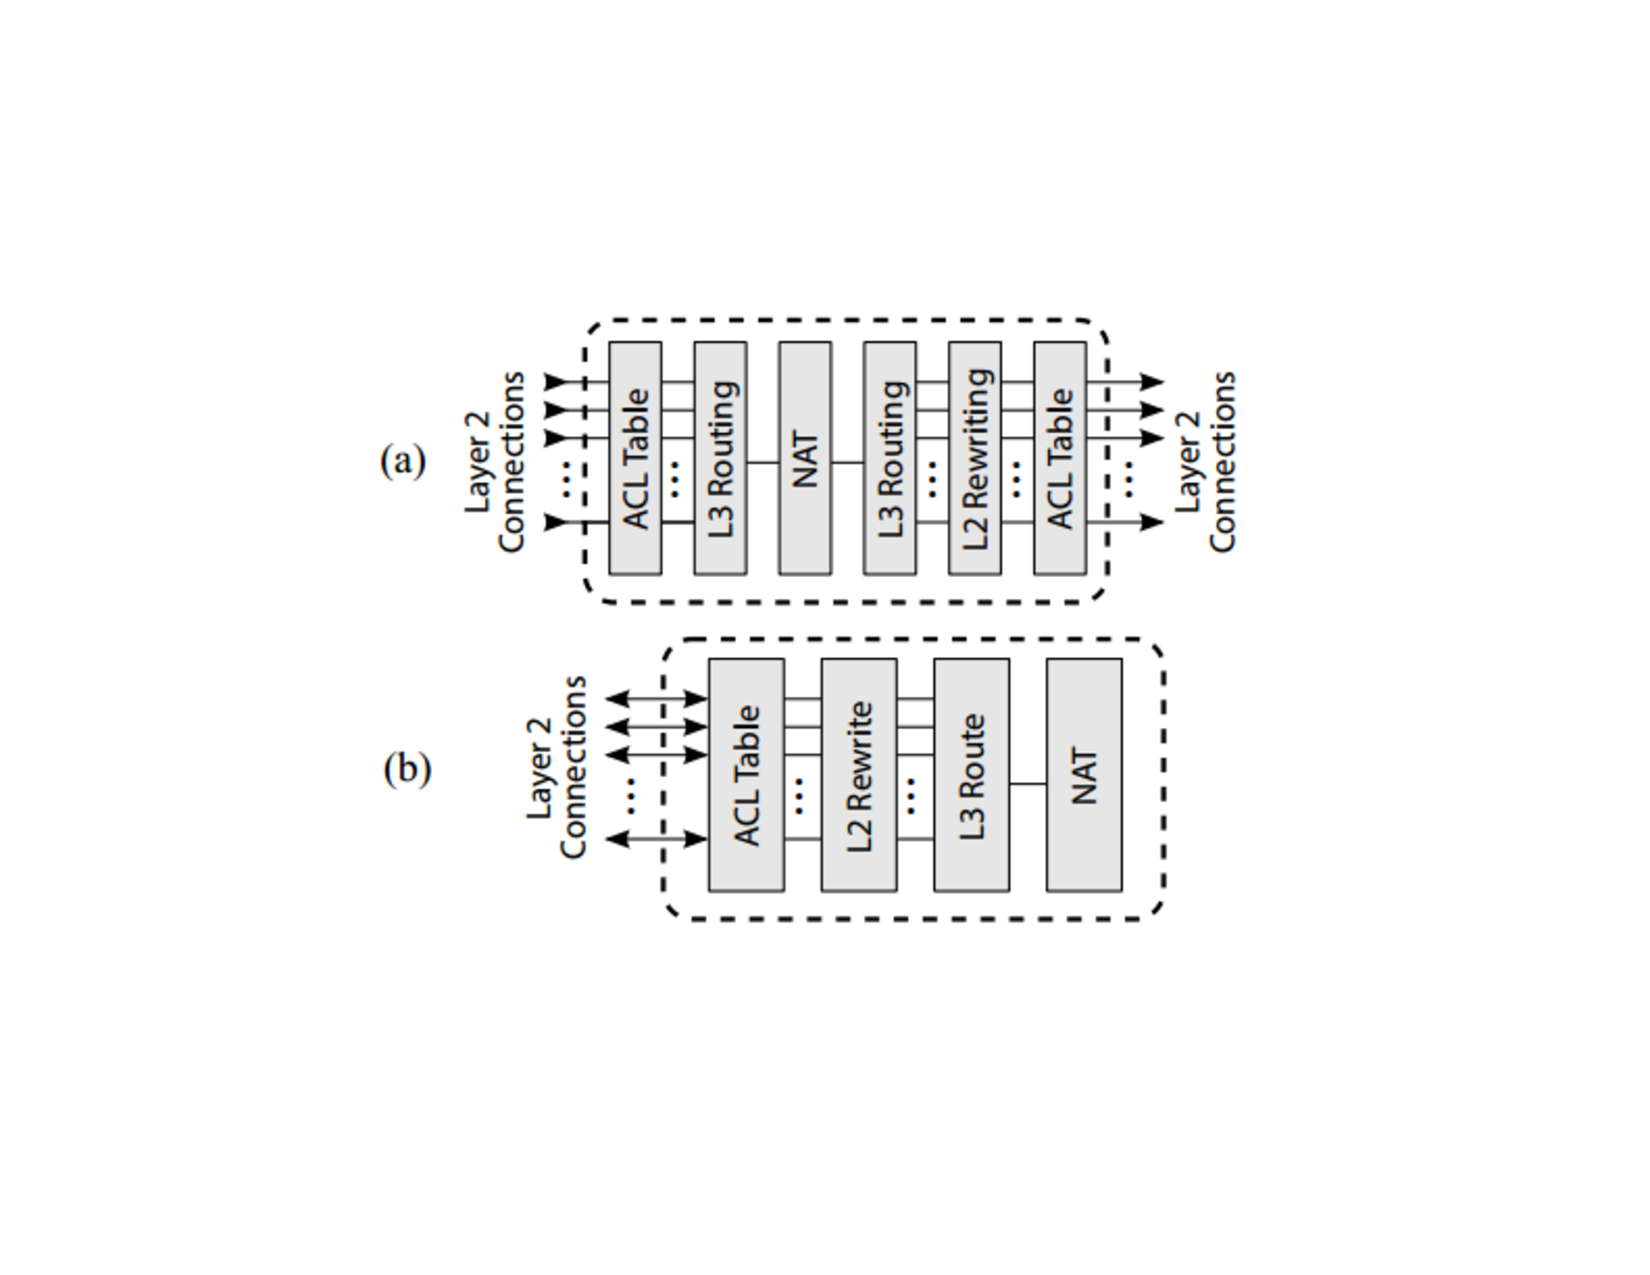
\includegraphics[width=0.7\textwidth]{ExodusRouter}
\vspace{-1.1in}
\caption{Logical flow tables in an Exodus router implementation(a), physical implementation with OpenFlow V1.0(b)}
\end{figure}
\par As we introduced above, we still have many questions that don't know how to solve. Also, due to the time limitation, in this project, we just verify the equivalence of the initial states of the two networks. The rest questions are open and will be our future work.

\section{Experiments and Results}
\par We think HSA should be better than ATPG to check the equivalence of the two initial states, because the initial state is a special network context. Meanwhile, this context is static and stable(some network contexts happen when the controller receive some kinds of packets). Based on current tools, we still need to do some work: 
\begin{itemize}
\item Currently, HSA can't parse flow tables in OpenFlow switches. We need to extend HSA to make it support OpenFlow.
\item Although both HSA and Exodus use Cisco IOS configuration files as input, the converting coverage of the two parsers are probably not the same(like NAT). We need to make and confirm the converting coverage in HSA and Exodus the same.
\item In Exodus, one original router or switch will be composed by wiring four single-table switches in series(as Fig. 1(b)). We need to compose the four transfer functions generated by HSA into one, like a big virtual switch. Meanwhile, we need to mapping the ports in the big virtual switch to the original ports to build the topology transfer functions. 
\end{itemize}

\par As we introduced above, the result of this project should be a set of network transfer functions($\Psi'$, correspond to each switches and routers) and topology network transfer functions($\Gamma'$, correspond to the network topology) of the Exodus generated SDN, like HSA. If we can prove that $\Phi^{'}(h,p)=\Psi'(\Gamma'(...(\Psi'(\Gamma'(h,p)...)$ equals to $\Phi^{k}(h,p)=\Psi(\Gamma(...(\Psi(\Gamma(h,p)...)$, we can conclude the two networks are equal.


%\begin{itemize}
%\item Lists
%\item Tables
%\item Math text
%\end{itemize}

%After you write your LaTeX source, you have to compile it, run
%BibTeX, and then compile twice again, to get all cross-references 
%right. I also included a Makefile to make that whole process easier.
%You just have to type \texttt{make} if you have your environment set.
%It should work on Linux, MacOS, and cygwin. If you are running 
%anything else, you should know how to set it up too.

%Some sample text. Paragraphs are created by blank lines in the source.
%Some sample text. Paragraphs are created by blank lines in the source.
%Some sample text. Paragraphs are created by blank lines in the source.
%Some sample text. Paragraphs are created by blank lines in the source.
%Some sample text. Paragraphs are created by blank lines in the source.

%Some sample text. Paragraphs are created by blank lines in the source.
%Some sample text. Paragraphs are created by blank lines in the source.
%Some sample text. Paragraphs are created by blank lines in the source.
%Some sample text. Paragraphs are created by blank lines in the source.
%Some sample text. Paragraphs are created by blank lines in the source.

%\section{Another Section}

%Another section. This one will have a figure. See
%Figure~\ref{fig:us-versus-them}. Each figure has a label, which must be
%defined \emph{after} the caption. Traditionally, people use
%\texttt{fig:...} for figure labels, \texttt{sec:...} for section
%labels, and \texttt{tab:...} for table labels. For example, this is a
%reference to Section~\ref{sec:intro}. 

%\begin{figure}
%\centering
%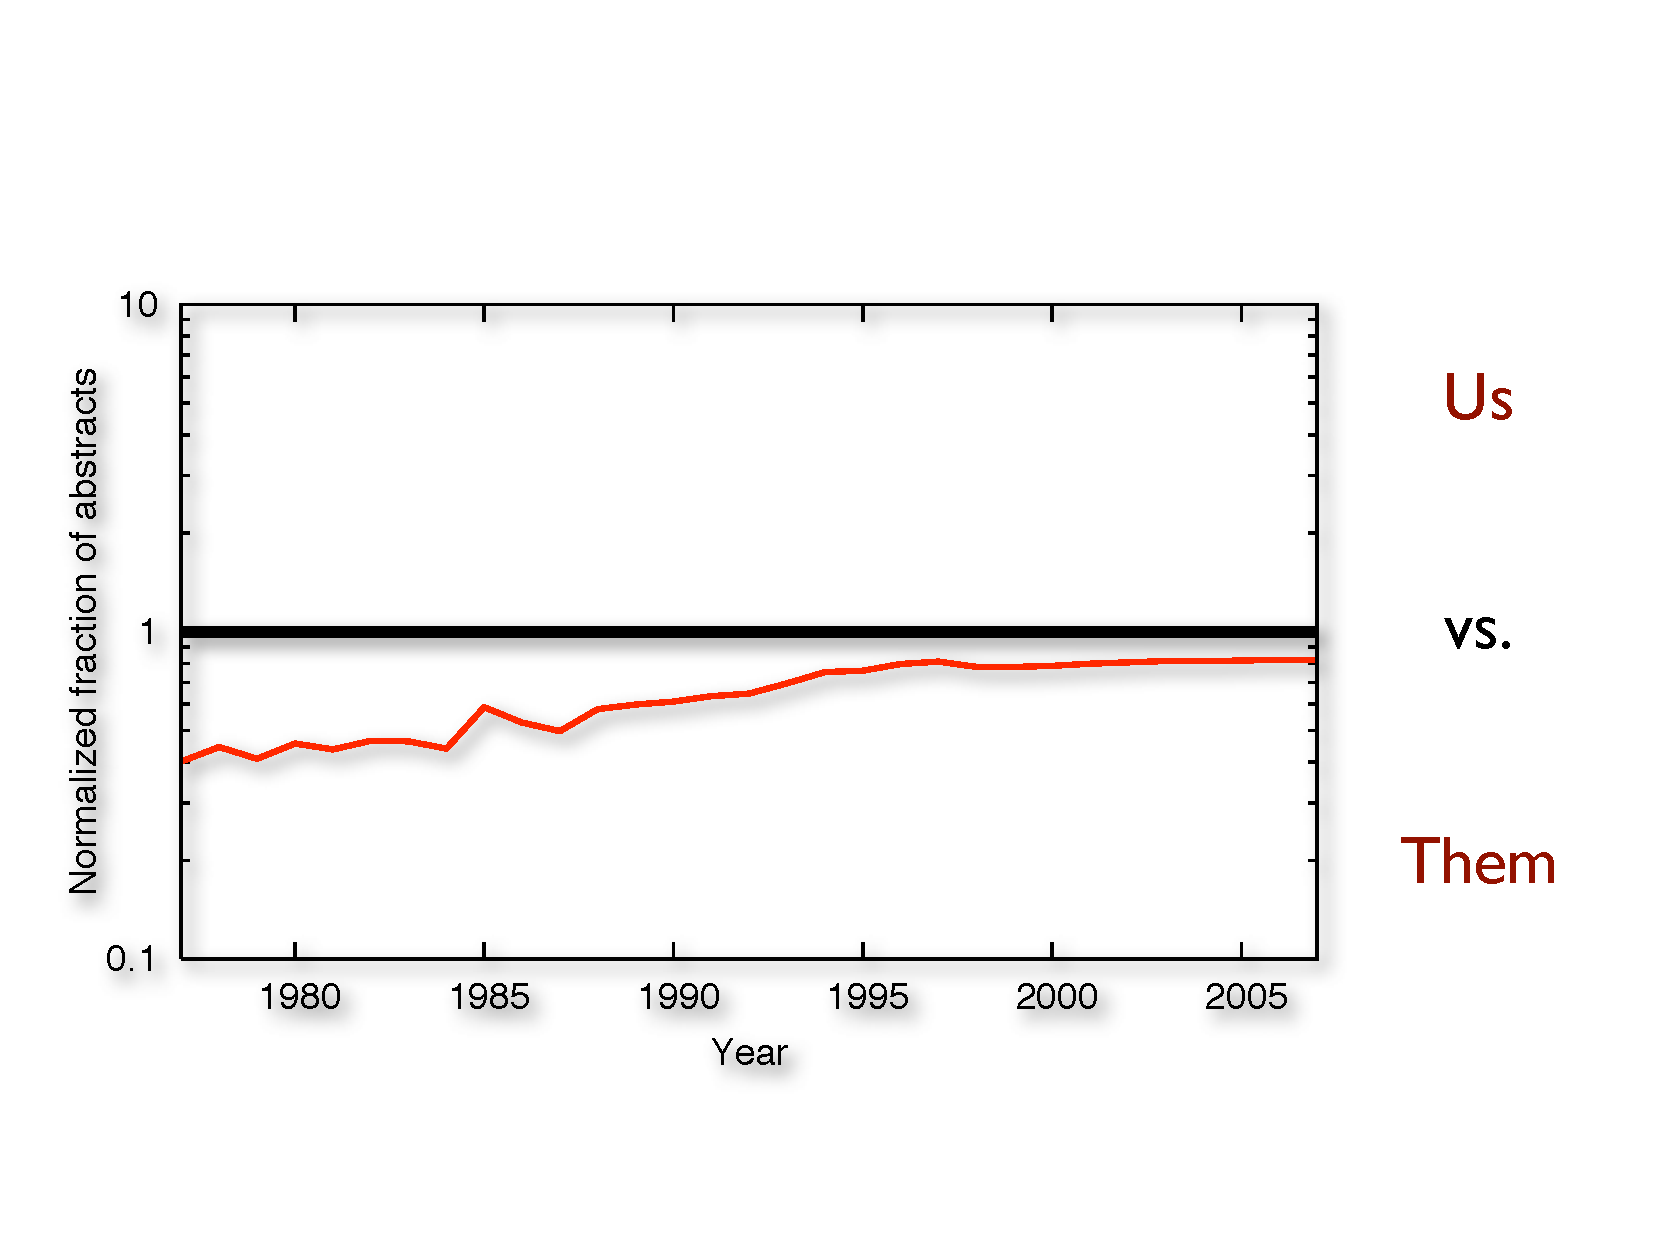
\includegraphics[width=0.7\textwidth]{usthem}
%\caption{Relative number of abstracts from the ACM Digital Library
%containing the word `us' versus the word 'them'. According
%to~\cite{godfrey08}, `they are winning, but we are gaining on Them'. }
%\label{fig:us-versus-them}
%\end{figure}

%\section{Related Work}

A nice feature for collaboration is that you can break your document
into many files with \texttt{\\input}, and have each person work on a
different file. This works great if you have some sort of version
control such as SVN or GIT.

Finally, you may want to cite some previous work. For
example,~\cite{lamport78time} is a highly-cited paper.
The ACM digital library is a good source of BibTeX entries.

% This is a comment: if you are curious, the ~ before \cite is a
% non-breaking space: it produces a space before the citation and
% doesn't let it go to the beginning of the next line if it would
% cause a line break.




%\section{Conclusions}

%It should be easy to write your report in LaTeX, and it's a great tool
%to learn. It almost certainly came with your Linux installation, and
%can be very easily installed in Cygwin and on the Mac (through the
%excellent MacTeX distribution).


%\bibliographystyle{plain}
%\bibliography{report}

\end{document}
